%! Author = adam
%! Date = 28.02.21

\chapter{Ion Beams in Semiconductor Physics}\label{ch:ion-beams-in-semiconductor-physics}
Another application of ion beams is their use in semiconductor physics.
Ion beams play a big role in the production of every day life technologies.
The transistors that sit within your phone or laptop are produced using ion beam implantation techniques.
The basics of this requires a basic understanding of semiconductor physics.
If we want to create integrated circuits, we are normally using silicon.
This is because of the energy band gap, $E_g$, between the conduction band and the valence band in the material.
For silicon, this energy band gap is about 1.12 eV.
Usually we use mono-crystalline silicon, and since it is a semiconductor, we will not have a high amount of charge carriers.
The higher the energy gap, the lower the intrinsic charge carrier density (see Fermi-Dirac statistics).
If we want to produce circuits, we can not use crystalline semiconductors, because there is too low intrinsic charge carrier density.
At room temperature, there is about $10^{10}$ charge carriers per cm$^3$, which is relatively low.
Without doping, the density of states (DOS), we have only little amount of holes in the conduction and valence bands, and is the same size for both.
There are several possibilities to produce higher charge concentrations in a semiconductor.
\section{Implantation}
\begin{wrapfigure}{r}{0.6\textwidth}
	\centering
	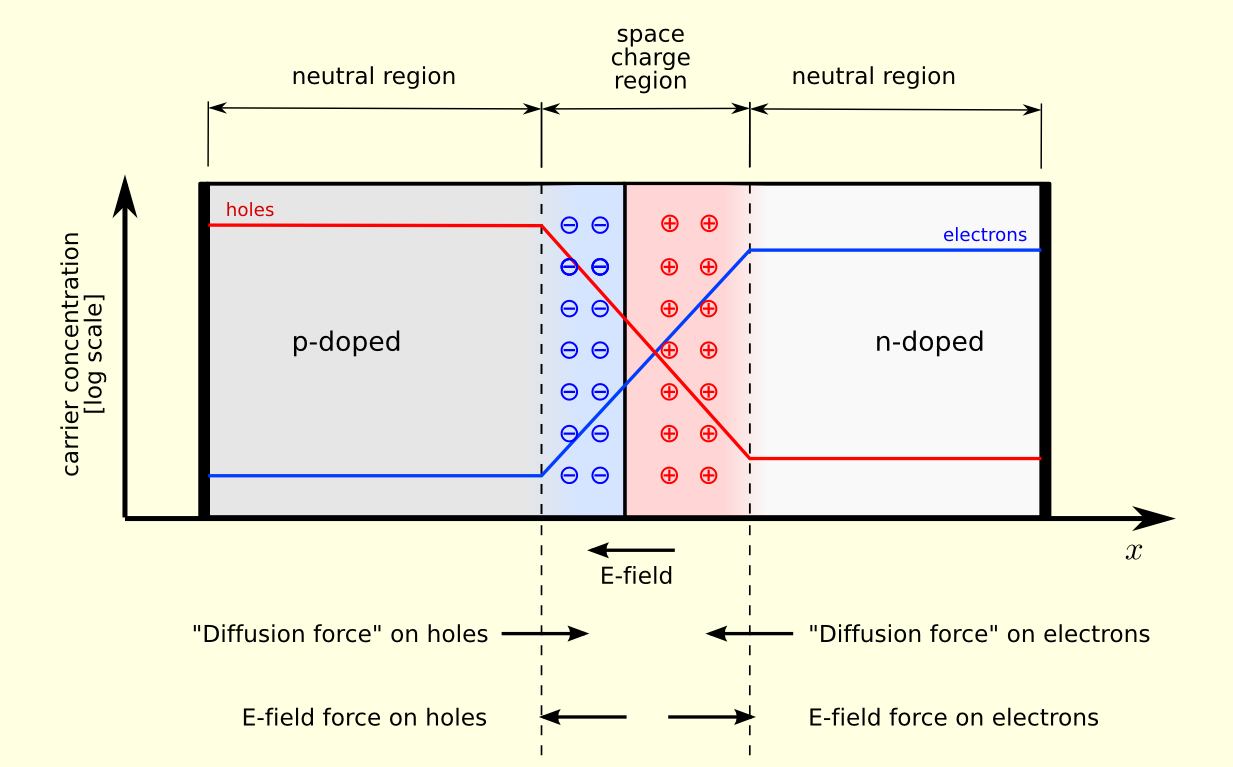
\includegraphics[scale=0.35]{pnjunc.png}
	\caption{A p–n junction in thermal equilibrium with zero-bias voltage applied. Electron and hole concentration are reported with blue and red lines, respectively. Gray regions are charge-neutral. Light-red zone is positively charged. Light-blue zone is negatively charged. The electric field is shown on the bottom, the electrostatic force on electrons and holes and the direction in which the diffusion tends to move electrons and holes.}
	\label{fig:pnjunc}
\end{wrapfigure}
We mentioned that with pure silicon crystals we have low charge carriers, so we could dope the silicon to tune the conductivity of the silicon.
In this process, we add another element other than silicon, for example arsenic, which has one electron more than silicon.
This additional electron can deliver itself to the conduction band, and we have a negative charge carrier, thus this type of silicon would be called \textbf{n-type}.
On the other hand, we could have positive charge carriers implanted, if for example we added boron to the lattice, which has one less electron, and thus one unbounded binding, i.e., we are missing an electron.
This results to a so-called mobile hole, and is almost like an electron with a positive charge, thus the name \textbf{p-type}.
With n-type we have thus much more electrons in the conduction band, because there is an increase in the DOS in the conduction band, and the shifting of the fermi energy towards this conduction band (for non-zero temperature, the fermi energy is replaced with the chemical potential).
One can play around with this kind of doping, an example is something called the PN junction found in Figure \ref{fig:pnjunc}.
We can use ion beam techniques to produce such p-n junctions!
By using ion beams, we can implement these dopants.
At some point there will be a middle point in the junction, in which the range of the n type ion beams and p type ion beams are the same, which you can see in the figure to the right.
So using the knowledge of the range of a particular ion beam in a sample, we can create certain levels in samples using different ion beams with varying energies (leading to different ranges), that can get increasingly sophisticated.
Implantation energies are typically 1keV to 1MeV.
The ion distributions have depths of between 10 nm to 10 $\mu$m.
Doses vary from $10^{12}$ ions per cm$^2$, and voltage adjustments in MOSFETs to 10$^{18}$ ions per cm$^2$ for formation fo buried insulating layers.
Methods of implantation can vary widely depending on the size of the sample.


\section{Annealing}
On the contrary to implantation, we have annealing, which is the process of repairing implant damage, i.e., 'healing' the surface by heating the sample.
Sometimes the process of implantation destroys other sites in the sample, thus necessitating a repair process after the implantation.
Not only does the repair the damage by the ions, but also puts the dopant atoms in substitution sites where they are electrically active.
There are generally two objectives/regimes of different temperature ranges for annealing.
One is the healing, or recrystallization, which is done in temperature ranges of 500--600 C.
The second is the renewing of electrical activity, 600--900 C.
As the lattice becomes repaired, the dopant atoms also fall into place in the lattice, and in the end we have a more or less perfect crystal just with various dopants spread across the lattice sites, adding electrons or holes depending on the doping.
The annealing process depends on the dopant type and dose.
For a given dose, annealing temperature is the temperature at which 90 percent of the implanted ions are activated by a 30-minute annealing in conventional furnace.
For example, boron needs a higher annealing temperature for higher doses.
At lower doses, p-type annealing is similar to n-type.
When the dose is greater than $10^{15}$ cm$^{-2}$, the annealing temperature drops to about 600C.
At doses greater than $6\times 10^{14}$cm$^{-2}$, the silicon surface becomes amorphous, and semiconductor underneath the amorphous layer is a seeding area for recrystallization.
For example, a 100--500 nm amorphous layer can be recrystallized in only a few minutes.
\section{Crystal Generation}
Using Cesium sputtering, we can get negatively charged ions and implant them into a silicon lattice, destroying the crystal order.
There are various regimes about this process, for example, some implanted ions will sputter away intrinsic ions, while in other cases the ions will just be implanted without erosion.
Based on the implantation energy of the ion, we have different sputtering yields, i.e., replacing intrinsic atoms with ions.
We are interested in this to see how different crystals can be created using these techniques.
We could then replace single target atoms with specific ions we want, i.e., building your own specialized lattice, and isotopically enriching layers.
An important result from this is that when combined with annealing, we can decrease spin noise, and increase coherence times (useful for quantum computing).
\section{Summary}
\begin{myitemize}
	\item Using ion beams, we know exactly how deep an ion will penetrate into a sample (range) and thus can construct diodes like p-n junctions
	\item We could also repair these devices using heating (annealing)
	\item we can generate crystals using ion beams, and combine these methods with annealing to get better coherence times and decrease spin noise.
\end{myitemize}
